\[
\bar{x} = t\bar{p} + (1 - t)\bar{q}
\]

\begin{tabular}{|>{\centering\arraybackslash}m{3.5cm}
                |>{\centering\arraybackslash}m{3.5cm}
                |>{\centering\arraybackslash}m{3.5cm}
                |>{\centering\arraybackslash}m{3.5cm}|}
\hline
\textbf{Line ($t \in \mathbb{R}$)} &
\textbf{Ray ($t \geq 0$)} &
\textbf{Line segment ($0 \leq t \leq 1$)} &
\textbf{Between ($0 < t < 1$)} \\
\hline


% 1. Line
\vspace{1em}
\begin{tikzpicture}
\draw[{Stealth[length=3mm, width=2mm]}-{Stealth[length=3mm, width=2mm]}] (-1.2,0) -- (1.2,0);
\fill (-0.7,0) circle (2pt) node[below] {$\bar{q}$};
\fill (0.7,0) circle (2pt) node[below] {$\bar{p}$};
\end{tikzpicture} &

% 2. Ray
\vspace{1em}
\begin{tikzpicture}
\draw[-{Stealth[length=3mm, width=2mm]}] (-0.7,0) --(1.2,0);
\fill (-0.7,0) circle (2pt) node[below] {$\bar{q}$};
\fill (0.7,0) circle (2pt) node[below] {$\bar{p}$};
\end{tikzpicture} &

% 3. Line segment
\vspace{1em}
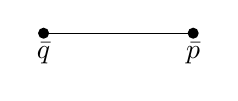
\begin{tikzpicture}
\draw[-] (-0.7,0) -- (1.2,0);
\fill (-0.7,0) circle (2pt) node[below] {$\bar{q}$};
\fill (1.2,0) circle (2pt) node[below] {$\bar{p}$};
\end{tikzpicture} &

% 4. Between
    \vspace{1em}
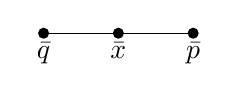
\begin{tikzpicture}
\draw[-] (-0.7,0) -- (1.2,0);
\fill (-0.7,0) circle (2pt) node[below] {$\bar{q}$};
\fill (0.25,0) circle (2pt) node[below] {$\bar{x}$};
\fill (1.2,0) circle (2pt) node[below] {$\bar{p}$};
\end{tikzpicture} \\

\hline
\end{tabular}
